\documentclass[conference]{IEEEtran}
\IEEEoverridecommandlockouts
% The preceding line is only needed to identify funding in the first footnote. If that is unneeded, please comment it out.
\usepackage{cite}
\usepackage{amsmath,amssymb,amsfonts}
\usepackage{algorithmic}
\usepackage{graphicx}
\usepackage{textcomp}
\usepackage{xcolor}
\usepackage{mathtools} 
\graphicspath{{../results/}}
\def\BibTeX{{\rm B\kern-.05em{\sc i\kern-.025em b}\kern-.08em
    T\kern-.1667em\lower.7ex\hbox{E}\kern-.125emX}}
\begin{document}

\title{Skull Stripping for MRI: a deep Convolution Neural Network approach}

\author{\IEEEauthorblockN{Kaiyuan(Eric) Chen}
\IEEEauthorblockA{\textit{Computer Science Department} \\
\textit{University of California, Los Angeles}\\
Los Angeles, United States \\
chenkaiyuan@ucla.edu}
\and
\IEEEauthorblockN{Jingyue Shen}
\IEEEauthorblockA{\textit{Computer Science Department} \\
\textit{University of California, Los Angeles}\\
Los Angeles, United States \\
brianshen@ucla.edu}
}

\maketitle

\begin{abstract}
In this work\footnote{Our implementation is on https://github.com/KeplerC/MRI-Skull-Stripping. More information can also be found on http://kychen.xyz/2018/06/02/MRI-2018/.}, we developed a deep Convolutional Neural Network(CNN) scheme to perform brain skull stripping on Magnetic Resonance Image(MRI). We analyzed previous works that employ machine learning algorithm including ensembled learning and linear models. By conducting series of experiments, we find weaknesses of those popular machine models like poor scalability and strong assumption on structure of images. In order to reduce above problems, we propose a CNN approach borrowed from autoencoders. Making use of the sparsity of images, we encode it to a more compact embedding and training a decoder to images with skull stripped. By experiments, we reach a higher scalability and better visual accuracy. 

\end{abstract}

\begin{IEEEkeywords}
Medical Imaging, Machine Learning, Skull Stripping, MRI
\end{IEEEkeywords}

\section{Introduction}
Computer aided diagnosis based on medical images from MRI(magnetic resonance image) has gained ubiquitous usage for its “noninvasive, nondestructive, flexible” properties[2]. With the help of FLAIR(Fluid-attenuated inversion recovery), Diffusion-weighted(DW) MRI, people can get an anatomical structure of human soft tissues with high resolution. Especially to satisfy the demand for interior and exterior structure of brain structures, MRI can produce cross-sectional images from different angles, for example, top-down, side-to-side and front-to-back: however, having slices from different angles give a lot of challenges in stripping those tissues which people are interested in, from xtra-cranial or non-brain tissues that has nothing to do with brain diseases such as Alzheimer’s disease, aneurysm in the brain, arteriovenous malformation-cerebral and Cushings disease and etc[1]. 

As a preliminary step for further analysis, brain segmentation, i.e. skull stripping, needs both speed and accuracy in practice, which should be considered in any algorithms proposed. By Kalavathi et al. [2], they can be classified into five categories: mathematical morphology-based methods, intensity-based methods, deformable surface-based methods, atlas-based methods, and hybrid methods. However, as we further reviewed on state-of-arts that are vaguely described in hybrid methods, we believe machine learning-based methods should also have its own place in brain segmentation. Machine learning is a broad concept that include many interesting algorithms that we would like to implement and experiment on. For example, Butman introduced a robust machine learning method that detects the brain boundary by random forest[2]. As random forest has high expressive power on voxels of brain boundary, this method can reach an high accuracy robustly. Popular methods like deep learning can also applied. For example, Kleesiek et al.[8] used non-parametric 3D Convolutional Neural Network(CNN) to learn important features and reach the highest Dice score among all the methods we have reviewed. However, as a parametric algorithm, GMM also has its place in brain segmentation. For example, Yunjie et al. developed a skull stripping method with an adaptive gauss mixture model and a 3D mathematical morphology method. The GMM is used to classify brain tissues and to estimate the bias field in the brain tissues [5]. These methods, along with well-implemented libraries such as sklearn[6], Tensorflow[7], are readily available for our use.

Our contribution in this work is as following:
\begin{itemize}
\item We conducted a series of experiments on previous works of machine learning based skull stripping, including ensembled learning like random forest and linear models like support vector machine(SVM). Then we analyze their weaknesses from observation. 
\item To solve problems of previous works, we adopt Convolution Neural Network(CNN) in a scheme similar to autoencoder. 
\item We manually labelled more than 700 MRI images. As previous sklearn-based works focus heavily on structure of image(pixel color, position and color of surrounding pixel), we also labeled various MRI examples that previous models would fail. 
\end{itemize}

\section{Problem Formulation}
\subsection*{Problem Definition}
We formulate our problem in the following way: given an image as matrix $X$, we can view it as a sum of skull matrix $S$ and stripped matrix $X'$, with dimension $w$ and $h$, i.e.
\[
X = S + X'
\]
where
\[
S_{ij} = 
\begin{cases}
X_{ij} &\text{if it is skull} \\
0 &\text{otherwise}
\end{cases}
\]
and 
\[
X'_{ij} = 
\begin{cases}
0 &\text{if it is skull} \\
X_{ij} &\text{otherwise}
\end{cases}
\]
and $X'_{ij}$ should be an output of our program. What we want is to optimize the following objective: 
\begin{equation}
\label{loss}
J(X') = \alpha{|X_{ij} -X'_{ij}|_2} + |S_{ij} - X'^c_{ij}|_2
\end{equation}
where $\alpha$ is a hyperparameter that can regularize the loss function and prevent overfitting. In this case, because brain stripping is a preprocessing step, we tend to penalize more to keep original brain structure the same, so we need a higher $\alpha$. 

\subsection{Data Preparation}
We used a software named OsiriX to perform manual skull stripping. We successfully stripped about 700 images to serve as ground truth data.


\section{Baseline Model}
There are many ways to solve the problem, both in terms of discriminative models and generative models. For all the baseline models in this paper, one can calculate 
\begin{equation}
\label{prob}
P(S_{ij} = 0 | i, j, X_{ij}, \{X_{mn}\}_{d((m,n), (i, j)) < \varepsilon})
\end{equation}
where d is a self-defined distance metric and $\varepsilon$ is a predefined patch size. 

\subsection{A comparison of Baseline Models}
Because of the limitation of this report, we cannot elaborate on how each method works. We deliberately choose three popular methods that fit to calculate equation \ref{prob} with a loss function of equation \ref{loss}. We adopted three methods:
\begin{itemize}
\item Logistic Regression: a basic linear model that models $P(\text{label|features})$ by a linear combination of features
\item Random Forest: a classic method for ensembled learning, which contains a bag of weak classifiers that conducts a vote for the final label
\item Support Vector Machine(SVM): a linear model that draws a hyperplane between positive and negative examples.
\end{itemize}
and we train it with all the training set by sklearn models, and compare by prediction accuracy of equation \ref{prob}. 

For the visibility of variance and small differences between other models, we have to scale it by putting logistic regression scores behind the legend. However, the pattern is pretty clear: logistic regression seems to have weak expressive power and cannot be trained with so many data; The random forest approach has lower cross validation score at the beginning, maybe because the expressive power is too high that it overfits the dataset. 

\subsection{Feature Selection}
From a input data perspective, there are three major popular methods
\begin{itemize}
\item pixel-based. Choosing $\varepsilon = 0$ and only select features based on itself.
\item patch-based. This method is the most popular for its scalability, by which one can choose distance to be Eulcidean distance or Manahttan distance and tune a self-defined $\varepsilon$ as a hyperparameter. 
\item image-based. One simply feeds the whole image in. Larger $\varepsilon$ usually requires more computational power. CNN method proposed in section IV will be image-based.
\end{itemize}
We conducted a series of experiments that show the difference on choosing features and $\varepsilon$. We performed random forest on all training data and chose different features(only color, position with x and y and color of local patches), then we normalize it in terms of difference between the one with combined. After six rounds of experiments, we get a breakdown pie chart on error of each feature:


It is obvious patch color contains more information than others, but position and color also takes great portion and their sum is beyond patch color. 

\subsection{Analysis}
As we can see from above experiments, it seems to have overreliance on position and color itself, even their sum is more than the patch color. As a result, if we have the following image in figure 1, it will not work.
Because original picture has huge number of noise, when models like random forest is applied, local patch will not be fully expressive enough to cover this case, then it turns out to be a failure in Figure 2.

\section{CNN model}
\subsection*{Intuition}
We adopted a CNN approach similar to autoencoder:

We train encoder and decoder together and by compression and convolution, we remove the skull by optimizing equation \ref{loss}. 

Here we take a similar approach that tries to learn the most representative encoding of the brain structure by compressing and decompressing the given image using Convolutional Neural Network(CNN) model. 

\subsection*{Model Setup}
We adopt a basic CNN Autoencoder implementation. In encoder part of the model, we choose three convolution layers with three max pooling layers. For the decoder part, we use three convolution layers, three deconvolution layers and an extra reconstruction layer to reconstruct the input image. Note that since we need to reconstruct the skull-stripped images given full images as input, we choose the mean square error(MSE) between stripped images and reconstructed images as loss function, rather than the MSE of input and reconstructed images as used in autoencoders.
\subsection*{Training}
Due to the time consuming manual skull stripping process, we are only able to obtain about 700 original and stripped images as dataset. So we choose batch size to be 15 and the number of epoch to be 50 to train our model. We adopt a roughly 7-2-1 train-validation-test split to choose hyperparameters such as initial learning rate. And we found that learning rate $\alpha = 0.003$ gives best result. The image below is the loss during training process.\\

After many experiments, we find that our model is able to detect the region of brain in the image, but cannot reconstruct the stripped image with resolution as high as the input. Since skull stripping is a preprocessing step for other diagnosis, which requires high resolution brain images, we use reconstructed images as bitmasks applied to unstripped images.
\subsection*{Testing}

The above images \ref{results} are some of our test results. The first row are original unstripped images. And second row are learned stripped images. As shown in those images, our algorithm can perform skull stripping well on various slices of brains.
In our dataset, each patient has about 20 brain images. Among all of patients, some of them have 1 to 2 images that are not stripped cleanly. The overall accuracy of our model is around $92\%$. One thing worth noting is that most of our model's inaccuracy comes from failing to strip a small portion of skull, as shown in the image below. In other words, the core brain parts remain intact, which is desirable for skull stripping.\\


\section{Conclusion and Future Work}
In this work, we compared and analyzed different machine learning models applied to skull stripping, including Logistic Regression, SVM and random forest. Because of their weakness in strong assumptions in dataset, they are not robust to circumstances with high noises or improperly aligned skulls. Then we propose a CNN approach that is similar to autoencoder, and with this scheme, we can remove those noises and be robust to new structures. 

However, as we acknowledged in previous section, it may fail to detect some parts of skull, and because of the nature of compression/reconstruction based model, it might have some loss in information on reconstructed image. As we already wrote 4 pages and requirement of this report should be 2 pages, we cannot cover more detailed experiments on how those reconstructed differ from original images and how those hyperparameters, like dropout, layers, will influence our results. We may do more and more rigorous experiments on CNN in the future. 

\begin{thebibliography}{00}
\bibitem{b1} G. Eason, B. Noble, and I. N. Sneddon, ``On certain integrals of Lipschitz-Hankel type involving products of Bessel functions,'' Phil. Trans. Roy. Soc. London, vol. A247, pp. 529--551, April 1955.\\
\bibitem{b2} Kalavathi,P. and V.B. Surya Prasath. ``Methods on Skull Stripping of MRI Head Scan Images -- a Review.'' Advances in Pediatries., U.S. National Library of Medicine, June 2016, www.ncbi.nlm.nih.gov/pmc/articles/PMC4879034.\\
\bibitem{b3} Two-dimensional fast magnetic resonance brain segmentation. Suri JS IEEE Eng Med Biol Mag. 2001 Jul-Aug; 20(4):84-95.\\
\bibitem{b4} Butman J, Roy S, Pham D. Robust skull stripping using multiple MR image contrasts insensitive to pathology. NeuroImage . 2017;146:132-147.\\
\bibitem{b5} Yunjie C, Jianwei Z, Shunfeng W. A new fast brain skull stripping method, biomedical engineering and informatics. Tianjin: Proc. 2nd International Conference on Biomedical Engineering and Informatics, BMEI09; 2009.\\
\bibitem{b6} Scikit-learn: Machine Learning in Python, Pedregosa et al., JMLR 12, pp. 2825-2830, 2011.\\
\bibitem{b7} Martín, et al. “TensorFlow: Large-Scale Machine Learning on Heterogeneous Distributed Systems.” [1402.1128] Long Short-Term Memory Based Recurrent Neural Network Architectures for Large Vocabulary Speech Recognition, 16 Mar. 2016, arxiv.org/abs/1603.04467.\\
\bibitem{b8} Kleesiek J, Urban G, Hubert A, Schwarz D, Maier -Hein K, Bendszus M, Biller A. Deep MRI brain extraction: A 3D convolutional neural network for skull stripping. NeuroImage . 2016;129:460-469.

\end{thebibliography}

\newpage
\begin{figure}[h!]
\caption{Original Baseline image}
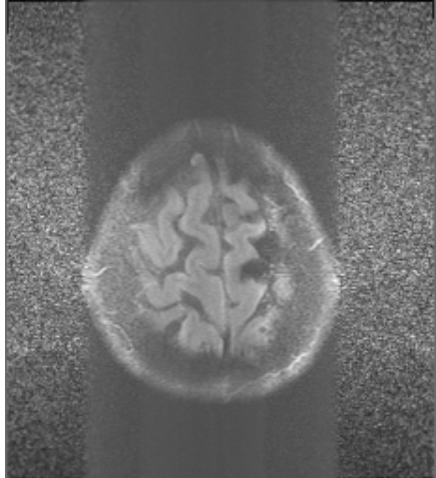
\includegraphics[scale = 0.34]{Snipaste_2018-05-28_14-39-56.png} 
\centering 
\end{figure}
\begin{figure}[h!]
\centering 
\caption{Processed Baseline image}
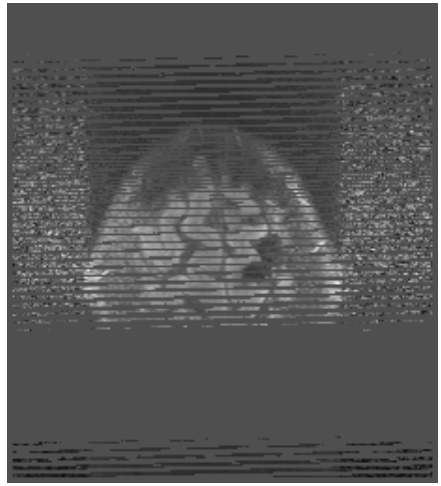
\includegraphics[scale = 0.34]{Snipaste_2018-05-28_14-40-00.png}
\end{figure}

\begin{figure}[h!]
\centering 
\caption{learning curve}
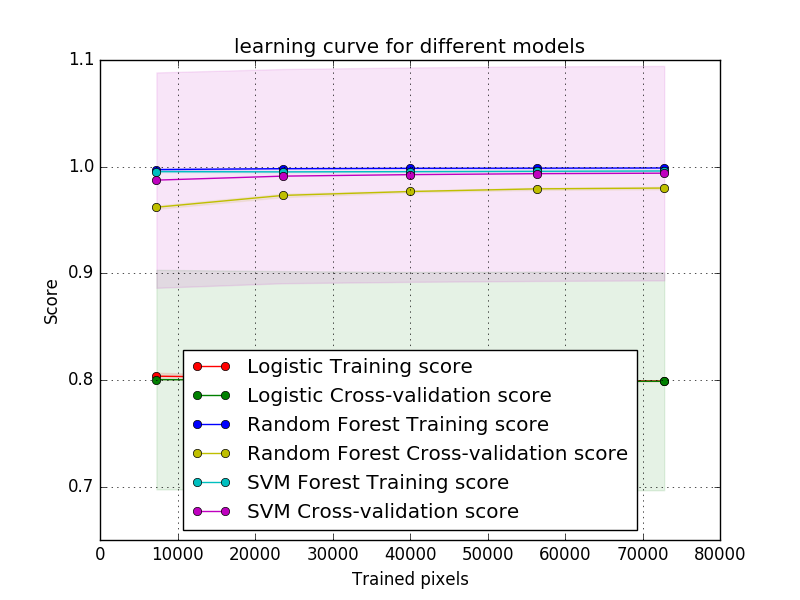
\includegraphics[scale = 0.4]{myfig.png}
\end{figure}


\begin{figure}[h!]
\centering 
\caption{A breakdown of errors with and without this feature}
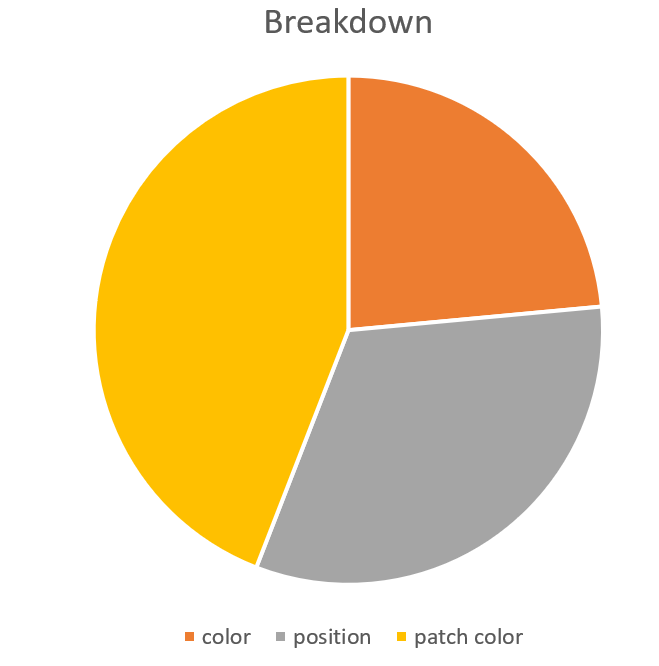
\includegraphics[scale = 0.4]{Snipaste_2018-05-28_13-52-29.png}
\end{figure}

\begin{figure}[h!]
\centering 
\caption{An illustration of our CNN scheme}
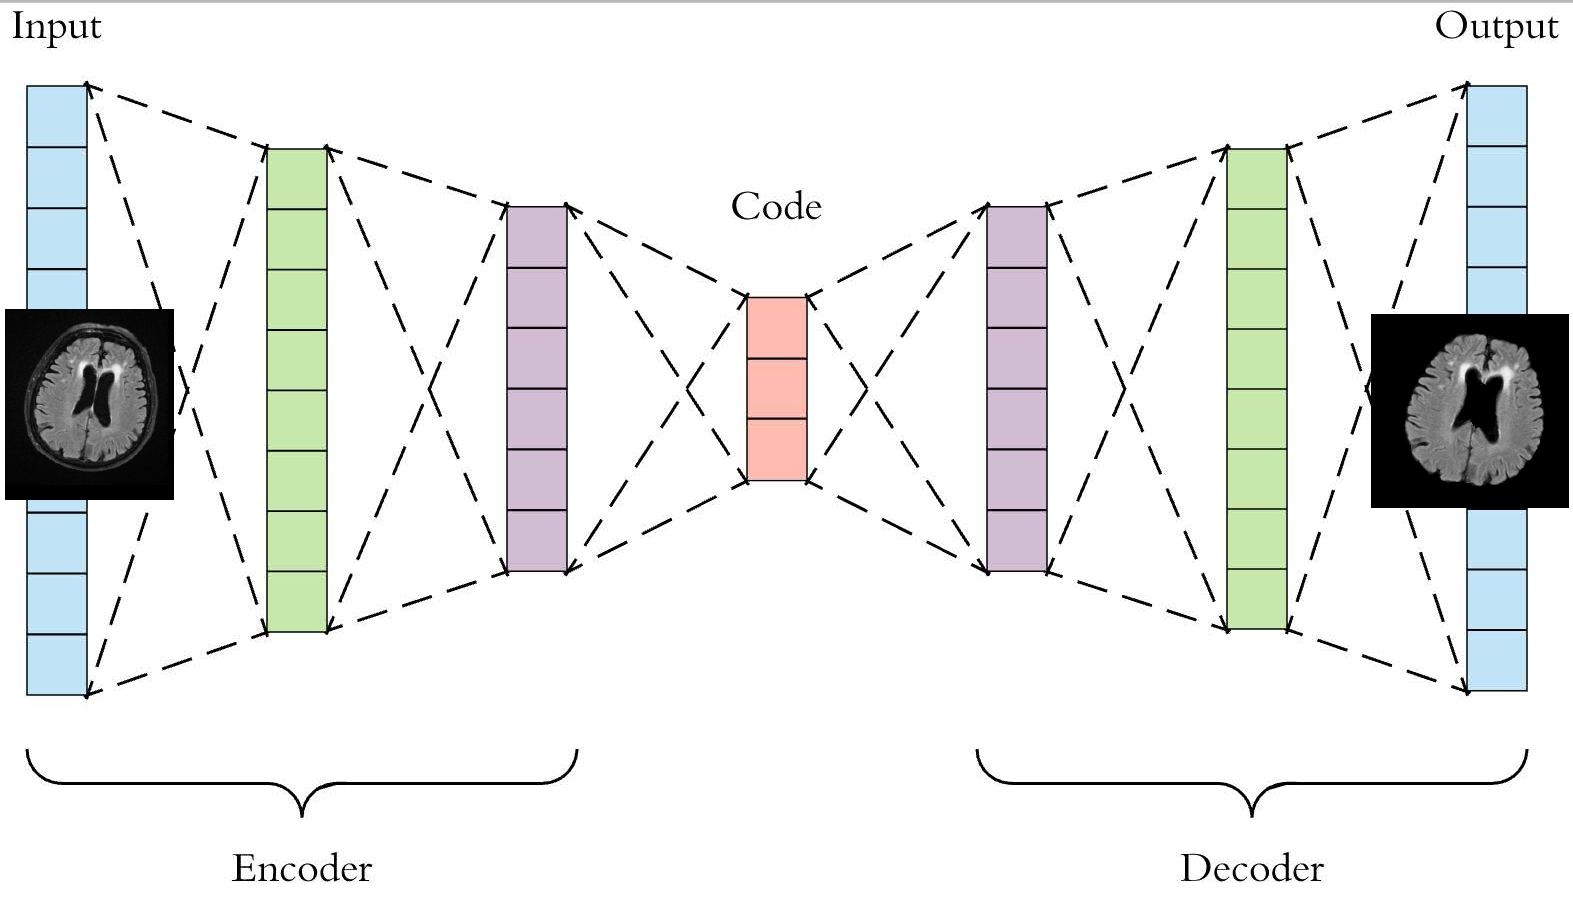
\includegraphics[scale = 0.3]{Snipaste_2018-05-28_14-16-23.png}
\end{figure}

\begin{figure}[h!]
\centering 
\caption{learning curve of CNN model}
    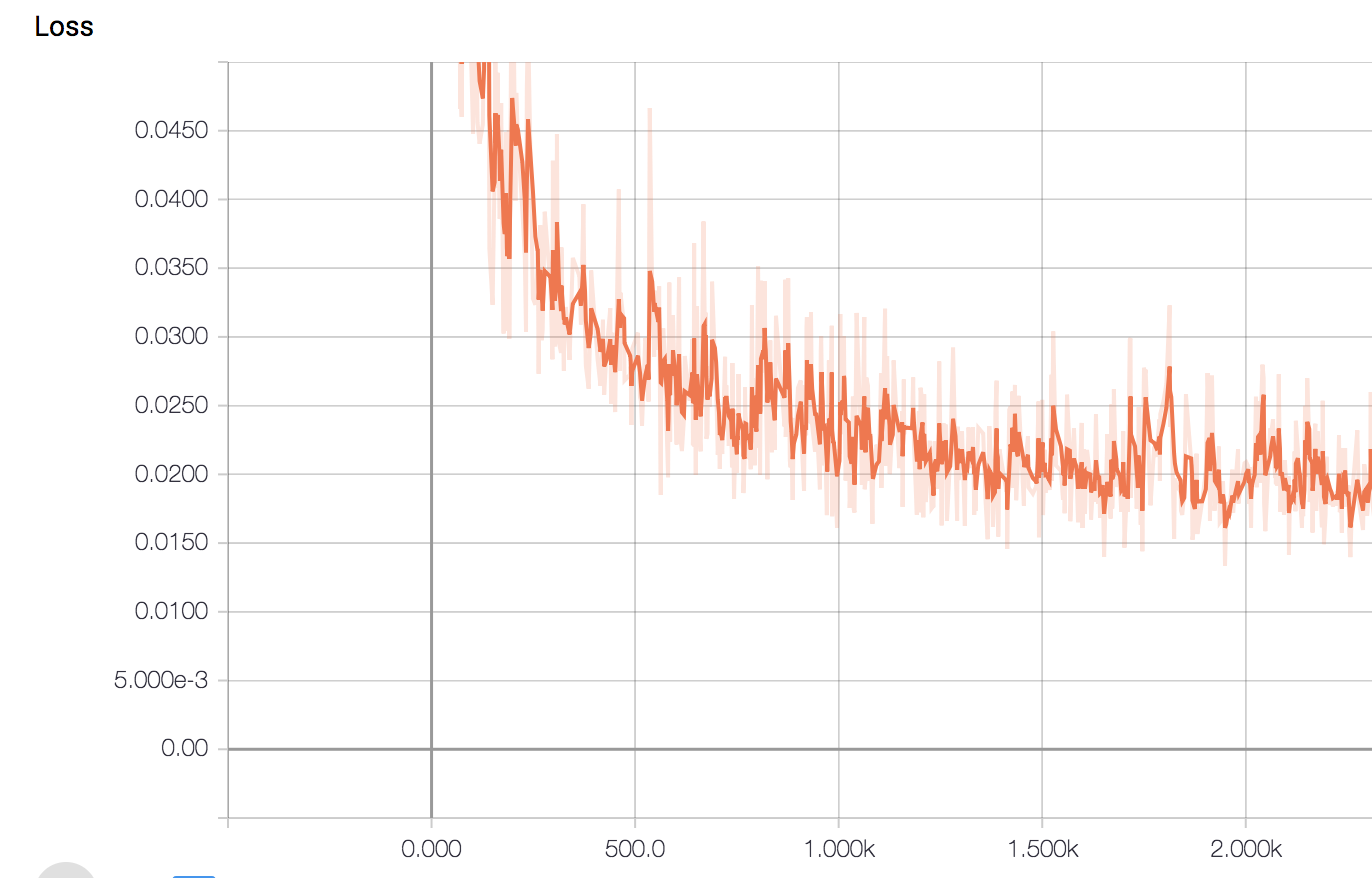
\includegraphics[scale=0.2]{loss.png}  
\end{figure}


\begin{figure}[h!]
\centering 
\caption{Our CNN results}
\label{results}
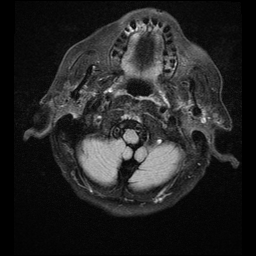
\includegraphics[scale = 0.2]{origin_0.png}
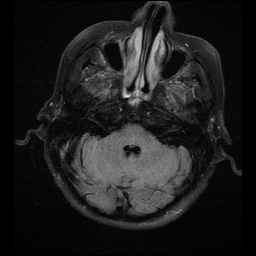
\includegraphics[scale = 0.2]{origin_4.png}
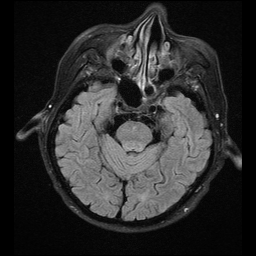
\includegraphics[scale = 0.2]{origin_6.png}
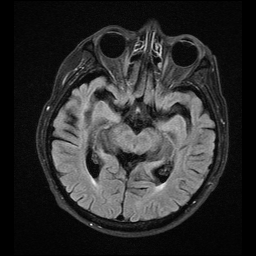
\includegraphics[scale = 0.2]{origin_9.png}
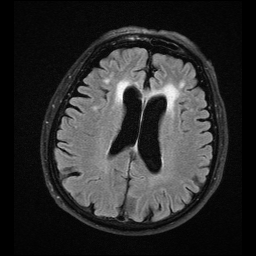
\includegraphics[scale = 0.2]{origin_14.png}
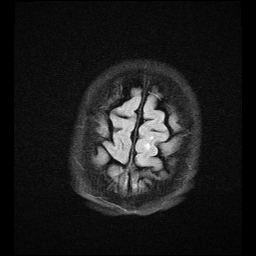
\includegraphics[scale = 0.2]{origin_21.png}

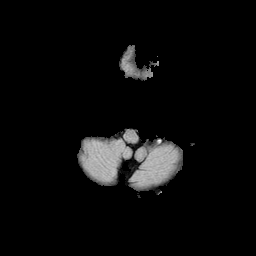
\includegraphics[scale = 0.2]{stripped_0.png}
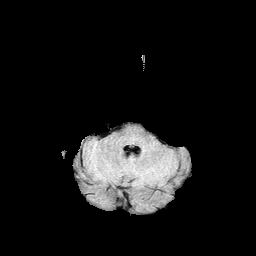
\includegraphics[scale = 0.2]{stripped_4.png}
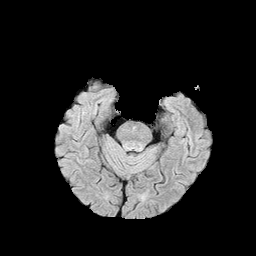
\includegraphics[scale = 0.2]{stripped_6.png}
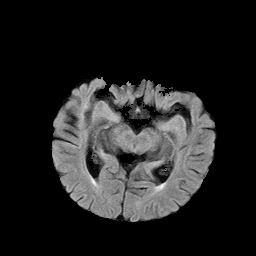
\includegraphics[scale = 0.2]{stripped_9.png}
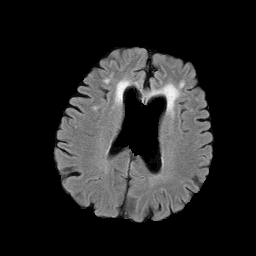
\includegraphics[scale = 0.2]{stripped_14.png}
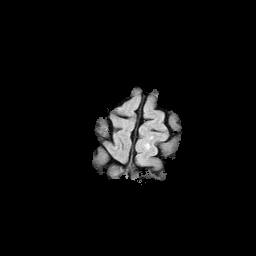
\includegraphics[scale = 0.2]{stripped_21.png}
\end{figure}

\begin{figure}[h!]
\centering 
\caption{Potential Errors on our model}

\hspace{8mm}
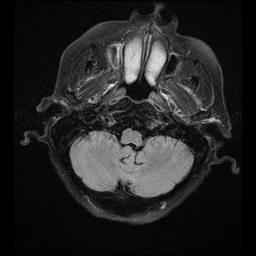
\includegraphics[scale = 0.3]{origin_2.png}
\hspace{22mm}
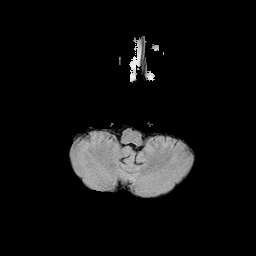
\includegraphics[scale = 0.3]{stripped_2.png}
\end{figure}





\end{document}
